% Ablation Study Boxplot across IEEE SPC, PPG-DaLiA, and WESAD (Fig. 6)
% Styled after original manuscript Fig. 5 with dashed horizontal grids and vertical dataset separators
% Compile: pdflatex fig_boxplot_A2.tex -> fig_boxplot_A2.pdf
\documentclass[border=4pt]{standalone}
\usepackage{tikz}
\usepackage{pgfplots}
\pgfplotsset{compat=1.18}
\usepgfplotslibrary{statistics}

\begin{document}
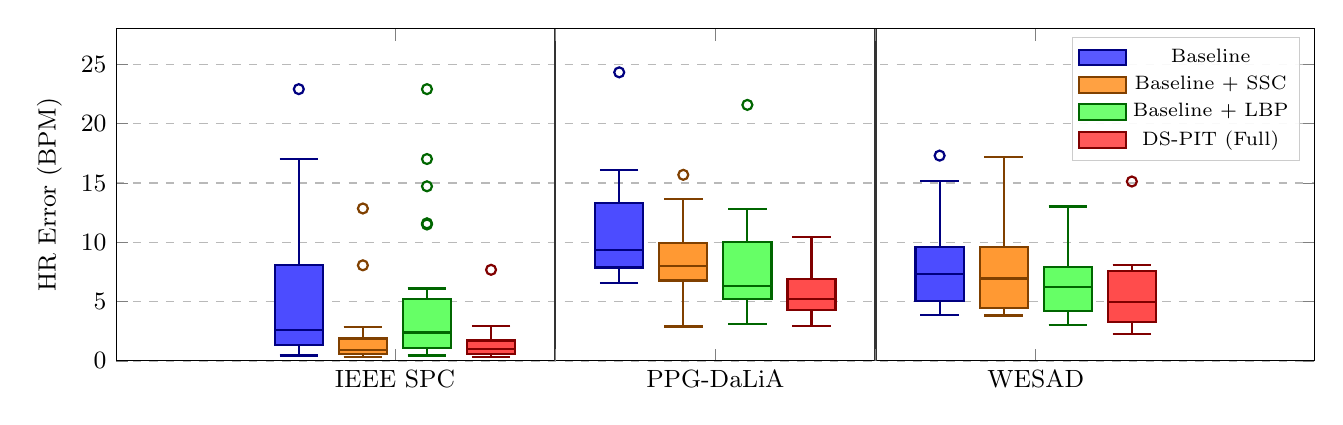
\begin{tikzpicture}
    \begin{axis}[
        width=16.8cm,
        height=5.8cm,
        ymin=0, ymax=28,
        ytick={0, 5, 10, 15, 20, 25},
        ylabel={HR Error (BPM)},
        xtick={1, 2, 3},
        xticklabels={IEEE SPC, PPG-DaLiA, WESAD},
        enlarge x limits=0.18,
        ymajorgrids=true,
        grid style={dashed, gray!55, line width=0.45pt},
        legend style={at={(0.988,0.975)}, anchor=north east, legend columns=1, font=\scriptsize, inner sep=2pt, row sep=-0.5pt, draw=gray!40, fill=white, fill opacity=0.92, text opacity=1},
        boxplot/draw direction=y,
        extra x ticks={1.5, 2.5},
        extra x tick labels={},
        extra x tick style={grid=major, major grid style={solid, thick, black!80}},
        tick label style={font=\small},
        label style={font=\small}
    ]
    
    % --- Legend Dummies ---
    \addplot [fill=blue!70!white, draw=blue!50!black, thick, area legend] coordinates {(0, -100)};
    \addlegendentry{Baseline}

    \addplot [fill=orange!80!white, draw=orange!50!black, thick, area legend] coordinates {(0, -100)};
    \addlegendentry{Baseline + SSC}

    \addplot [fill=green!60!white, draw=green!40!black, thick, area legend] coordinates {(0, -100)};
    \addlegendentry{Baseline + LBP}

    \addplot [fill=red!70!white, draw=red!50!black, thick, area legend] coordinates {(0, -100)};
    \addlegendentry{DS-PIT (Full)}

    % ================= IEEE SPC (n = 23) =================
    % IEEE SPC - Baseline (MAE = 5.56, med = 2.62)
    \addplot [
        fill=blue!70!white, draw=blue!50!black, thick,
        boxplot prepared={
            draw position=0.70,
            lower whisker=0.450, lower quartile=1.350, median=2.620, upper quartile=8.095, upper whisker=17.020,
            box extend=0.15
        },
        mark=o, mark size=1.8pt, mark options={color=blue!50!black, thick}
    ] coordinates {
        (0, 22.910)
    };

    % IEEE SPC - Baseline + SSC (MAE = 1.96, med = 0.91)
    \addplot [
        fill=orange!80!white, draw=orange!50!black, thick,
        boxplot prepared={
            draw position=0.90,
            lower whisker=0.340, lower quartile=0.605, median=0.910, upper quartile=1.885, upper whisker=2.860,
            box extend=0.15
        },
        mark=o, mark size=1.8pt, mark options={color=orange!50!black, thick}
    ] coordinates {
        (0, 12.850) (0, 8.060)
    };

    % IEEE SPC - Baseline + LBP (MAE = 4.97, med = 2.39)
    \addplot [
        fill=green!60!white, draw=green!40!black, thick,
        boxplot prepared={
            draw position=1.10,
            lower whisker=0.450, lower quartile=1.080, median=2.390, upper quartile=5.240, upper whisker=6.110,
            box extend=0.15
        },
        mark=o, mark size=1.8pt, mark options={color=green!40!black, thick}
    ] coordinates {
        (0, 22.910) (0, 17.020) (0, 14.720) (0, 11.500) (0, 11.600)
    };

    % IEEE SPC - DS-PIT (Full) (MAE = 1.50, med = 1.00)
    \addplot [
        fill=red!70!white, draw=red!50!black, thick,
        boxplot prepared={
            draw position=1.30,
            lower whisker=0.340, lower quartile=0.605, median=1.000, upper quartile=1.730, upper whisker=2.930,
            box extend=0.15
        },
        mark=o, mark size=1.8pt, mark options={color=red!50!black, thick}
    ] coordinates {
        (0, 7.680)
    };

    % ================= PPG-DaLiA (n = 15) =================
    % PPG-DaLiA - Baseline (MAE = 11.01, med = 9.35)
    \addplot [
        fill=blue!70!white, draw=blue!50!black, thick,
        boxplot prepared={
            draw position=1.70,
            lower whisker=6.565, lower quartile=7.880, median=9.349, upper quartile=13.342, upper whisker=16.094,
            box extend=0.15
        },
        mark=o, mark size=1.8pt, mark options={color=blue!50!black, thick}
    ] coordinates {
        (0, 24.326)
    };

    % PPG-DaLiA - Baseline + SSC (MAE = 8.69, med = 7.97)
    \addplot [
        fill=orange!80!white, draw=orange!50!black, thick,
        boxplot prepared={
            draw position=1.90,
            lower whisker=2.907, lower quartile=6.786, median=7.974, upper quartile=9.965, upper whisker=13.672,
            box extend=0.15
        },
        mark=o, mark size=1.8pt, mark options={color=orange!50!black, thick}
    ] coordinates {
        (0, 15.688)
    };

    % PPG-DaLiA - Baseline + LBP (MAE = 8.22, med = 6.33)
    \addplot [
        fill=green!60!white, draw=green!40!black, thick,
        boxplot prepared={
            draw position=2.10,
            lower whisker=3.119, lower quartile=5.198, median=6.333, upper quartile=10.008, upper whisker=12.838,
            box extend=0.15
        },
        mark=o, mark size=1.8pt, mark options={color=green!40!black, thick}
    ] coordinates {
        (0, 21.583)
    };

    % PPG-DaLiA - DS-PIT (Full) (MAE = 5.83, med = 5.23)
    \addplot [
        fill=red!70!white, draw=red!50!black, thick,
        boxplot prepared={
            draw position=2.30,
            lower whisker=2.916, lower quartile=4.296, median=5.225, upper quartile=6.908, upper whisker=10.443,
            box extend=0.15
        },
        mark=o, mark size=1.8pt, mark options={color=red!50!black, thick}
    ] coordinates {};

    % ================= WESAD (n = 15) =================
    % WESAD - Baseline (MAE = 8.28, med = 7.31)
    \addplot [
        fill=blue!70!white, draw=blue!50!black, thick,
        boxplot prepared={
            draw position=2.70,
            lower whisker=3.860, lower quartile=5.074, median=7.314, upper quartile=9.623, upper whisker=15.196,
            box extend=0.15
        },
        mark=o, mark size=1.8pt, mark options={color=blue!50!black, thick}
    ] coordinates {
        (0, 17.308)
    };

    % WESAD - Baseline + SSC (MAE = 7.83, med = 6.94)
    \addplot [
        fill=orange!80!white, draw=orange!50!black, thick,
        boxplot prepared={
            draw position=2.90,
            lower whisker=3.826, lower quartile=4.487, median=6.942, upper quartile=9.617, upper whisker=17.178,
            box extend=0.15
        },
        mark=o, mark size=1.8pt, mark options={color=orange!50!black, thick}
    ] coordinates {};

    % WESAD - Baseline + LBP (MAE = 6.54, med = 6.22)
    \addplot [
        fill=green!60!white, draw=green!40!black, thick,
        boxplot prepared={
            draw position=3.10,
            lower whisker=3.035, lower quartile=4.200, median=6.217, upper quartile=7.941, upper whisker=13.011,
            box extend=0.15
        },
        mark=o, mark size=1.8pt, mark options={color=green!40!black, thick}
    ] coordinates {};

    % WESAD - DS-PIT (Full) (MAE = 5.76, med = 4.97)
    \addplot [
        fill=red!70!white, draw=red!50!black, thick,
        boxplot prepared={
            draw position=3.30,
            lower whisker=2.236, lower quartile=3.307, median=4.965, upper quartile=7.572, upper whisker=8.091,
            box extend=0.15
        },
        mark=o, mark size=1.8pt, mark options={color=red!50!black, thick}
    ] coordinates {
        (0, 15.124)
    };

    \end{axis}
\end{tikzpicture}
\end{document}
